\documentclass[14pt]{article}
\usepackage{graphicx}

\begin{document}

ordering the citations \cite{hackD} \cite{Fortnow} \cite{Sipser} 

\section*{\textbf{P} $ = $ \textbf{NP} versus \textbf{P} $\neq$ \textbf{NP}}
\hspace*{.25cm} Time complexity applies to number theory, computer science, and combinatorics. Methods of encryption (\emph{i.e.} RSA, Diffie-Hellman Key Exchange, Elgamod, DSA) rely heavily on the \textit{hope} that \textbf{P} $\neq$ \textbf{NP}. Transactions with credit cards and sending other types of sensitive messages use complex encryption methods that use \textbf{LARGE} prime numbers. If \textbf{P} $ = $ \textbf{NP} then that means that exist methods to figure out and confirm what specific peoples' prime numbers use to encrypt and decrypt those messages quickly; which would imply that our entire economic systems would be built on a house of cards.\\
\newpage

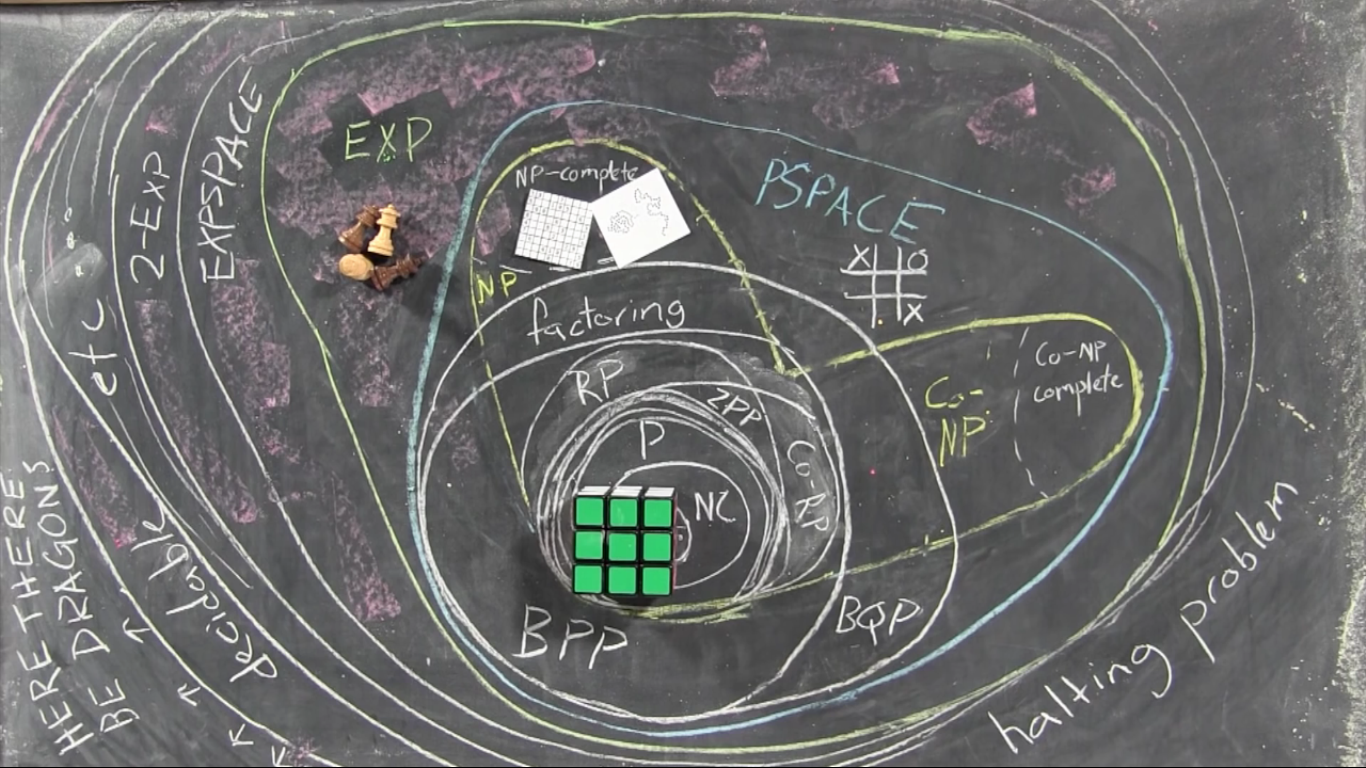
\includegraphics[scale=.45, angle = 90]{examples} \cite{hackD}\\



\bibliographystyle{plain}
\bibliography{references}


\end{document}